%%%%%%%%%%%%%%%%%%%%%%%%%%% asme2e.tex %%%%%%%%%%%%%%%%%%%%%%%%%%%%%%%
% Template for producing TSFP-format articles using LaTeX
% Based on the asme2e template (http://iel.ucdavis.edu/code/ASME/)
% Modified: 11 February 2013 for TSFP8 by R. Manceau
% Modified: 05 May 2014 for TSFP9&10 by K. Chauhan
% In case of problem: kapil.chauhan@sydney.edu.au
%%%%%%%%%%%%%%%%%%%%%%%%%%%%%%%%%%%%%%%%%%%%%%%%%%%%%%%%%%%%%%%%%%%%%%

%%%%%%%%%%%%%%%%%%%%%%%%%%%%%%%%%%%%%%%%%%%%%%
% To generate a pdf, compile either with pdflatex
% or with latex and
% dvips tsfp_template -Ppdf -t a4 -o
% followed by
% ps2pdf tsfp_template.ps
% (avoid using dvipdf that does not preserve the page layout on some systems)
%%%%%%%%%%%%%%%%%%%%%%%%%%%%%%%%%%%%%%%%%%%%%%

%%% use twocolumn and 10pt options with the tsfp format
\documentclass[twocolumn,10pt]{tsfp}
\usepackage{flushend}
\usepackage{graphicx}
\usepackage{color}
\usepackage{amssymb}
\usepackage{amsmath}
\usepackage{amssymb}
\usepackage[authoryear,round]{natbib}

\title{Instructions for TSFP-10 paper preparation using \LaTeX}

%%%% In case you need to slightly adapt the horizontal spacing between authors (for more than 3 authors) uncomment the following command
%%%% and if necessary modify the factor
%\renewcommand{\expauthors}{1.1}

%%% first author
\author{First Author
    \affiliation{
	Department of ...\\
	Organization/University\\
	Address\\
    email
    }	
}

%%% second author
%%% remove the following entry for single author papers
%%% add more entries for additional authors
\author{Second Author
          \affiliation{Department of ...\\
	Organixation/University\\
	Address\\
	email
    }
}


\begin{document}

\maketitle   %Print title matter

% Set the font to 9pt.
\fontsize{9}{11}\selectfont

%%%%%%%%%%%%%%%%%%%%%%%%%%%%%%%%%%%%%%%%%%%%%%%%%%%%%%%%%%%%%%%%%%%%%%
\section*{ABSTRACT}

This document is a template for preparing a manuscript for TSFP10 on Letter size paper.

The maximum length of the manuscript is six (6) pages.

Begin your abstract 115 mm from the top of the page as shown on this page. The ABSTRACT heading should be boldface in all capitals; it should be in a 9 pt. sans serif typeface (Helvetica) as shown above. It should be flush left with the left margin. The abstract text should be in 9 pt. New Times Roman font, the same as the main text. The spacing to the next heading should be two (2) line spaces.

%%%%%%%%%%%%%%%%%%%%%%%%%%%%%%%%%%%%%%%%%%%%%%%%%%%%%%%%%%%%%%%%%%%%%%
\section*{PAPER TITLE AND AUTHOR(S)}

The title should be boldface in all capital letters; it should be in a 12 pt. sans serif typeface (Helvetica) as shown above with 13 pt. leading (leading is the spacing between lines of text.) The title should be centered on the page, the longest line not to exceed 150 mm. All lines (including run-over lines of a long title) should be centered. Three (3) line spaces separate the title from the first author. Author name should consist of first name, middle initial, last name. It should be boldface, upper and lower case letters (with 12 pt. leading), centered under the title. Author affiliation should consist of the following as applicable and in the order noted:

\begin{itemize}
\item[$\bullet$] department or division name
\item[$\bullet$] company or university name
\item[$\bullet$] postal address, city, state or province name (spelled out), postal or zip code and country name
\item[$\bullet$] email of author
\end{itemize}

All author names and affiliation information should be 10 pt. Helvetica medium, upper and lower case letters (with 12 pt. leading), centered under the name. Two (2) line spaces separate the first and subsequent authors.

%%%%%%%%%%%%%%%%%%%%%%%%%%%%%%%%%%%%%%%%%%%%%%%%%%%%%%%%%%%%%%%%%%%%%%
\section*{TEXT HEADING \#1}

The text of the paper follows the abstract and should be set in 9 pt. New Times Roman font with default leading of 11pt. leading. The text should be 78 mm wide and justified on the right and left margins. The first line of each paragraph should be indented two spaces from the left margin. The text should be arranged in a two-column format as shown on this page. The primary text heading (text heading \#1) should be 9 pt. Helvetica boldface in all capitals, flush left with the left margin. If the heading should run to more than one line, the run-over text should also be flush left. The spacing to the next heading should be two (2) line spaces.

%%%%%%%%%%%%%%%%%%%%%%%%%%%%%%%%%%%%%%%%%%%%%%%%%%%%%%%%%%%%%%%%%%%%%%
\subsection*{Text Heading \#2}

The next level of heading should be 9 pt. Helvetica boldface, upper and lower case letters. The heading is flush left with the left margin. The spacing to the next heading should be two (2) line spaces.

%%%%%%%%%%%%%%%%%%%%%%%%%%%%%%%%%%%%%%%%%%%%%%%%%%%%%%%%%%%%%%%%%%%%%%
\subsubsection*{Text Heading \#3}

The third level of heading should follow the style of text heading \#2, but it will be indented and followed by a period, a space, and its text.

%%%%%%%%%%%%%%%%%%%%%%%%%%%%%%%%%%%%%%%%%%%%%%%%%%%%%%%%%%%%%%%%%%%%%%
\section*{PAGE NUMBERS}

Number the pages at the bottom center, as shown in the template.

%%%%%%%%%%%%%%%%%%%%%%%%%%%%%%%%%%%%%%%%%%%%%%%%%%%%%%%%%%%%%%%%%%%%%%
\section*{FOOTNOTES}

Footnotes should be numbered consecutively using superscript numbers\footnote{This is footnote number one.}. They should be positioned flush left at the bottom of the column in which the reference first appears\footnote{This is the second footnote.}. The width should not exceed the dimensions of the column width. The footnote should be preceded by a thin line. The text of the footnote should be 8 pt. Times New Roman font with 10 pt. leading. There should be one (1) line space between the line and the text.

%%%%%%%%%%%%%%%%%%%%%%%%%%%%%%%%%%%%%%%%%%%%%%%%%%%%%%%%%%%%%%%%%%%%%%
\section*{EQUATIONS/FORMULAE}

Equations should be centered in the column with two or three line spaces to separate equations from text. They also should be numbered consecutively, using Arabic numerals enclosed in parentheses and positioned flush right along the final baseline of the equation. Do not include any ellipses (dots) from the equation to the equation number, or any punctuation at the end of the equation itself.

Example:

\begin{equation}
F(x) = \int_{-\infty}^x f(x) \mathrm{d}x
\label{eq_1}
\end{equation}

%%%%%%%%%%%%%%%%%%%%%%%%%%%%%%%%%%%%%%%%%%%%%%%%%%%%%%%%%%%%%%%%%%%%%%
\section*{FIGURES AND PHOTOGRAPHS}

All figures, graphs and line drawings should be clear and sharp and of high quality (photocopies are not acceptable). Color figures are allowed. Figures may be placed either at the end of the paper or within the text of the paper, in the same page as the first reference of the figure, or the following page if there is not adequate space. If figures are placed within the text of the paper, it is preferable to position them at the top of the page. All figures should be in place when your paper is submitted.

Photographs should be of good quality, in black and white or color and camera ready. Photographs, like figures, should be placed directly on the page, at the end of the paper or within the text of the paper. Photographs should be sized to accurately meet the page specifications.

All figures/photographs should be numbered consecutively and captioned. The caption should be 9 pt, and upper and lower case letters, and centered under the figure/photograph. All callouts/text within the figure should be no smaller than 7 pt when sized to fit the column.
There should be a minimum of two line spaces between figures/photographs and text.


	\begin{figure}[t]
	\centering
	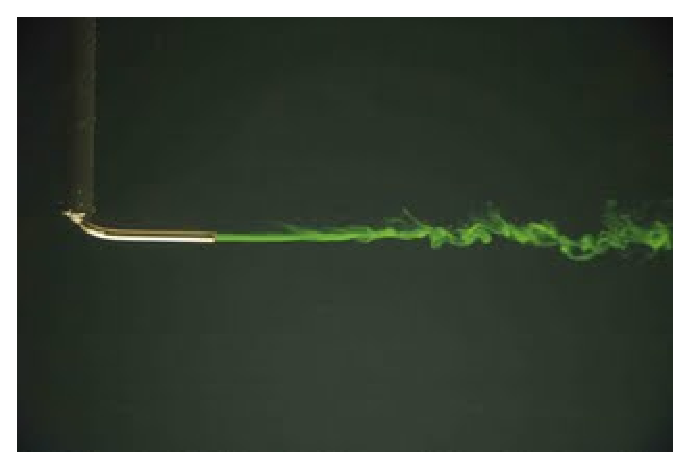
\includegraphics[width=3in]{SampleImage1}
	\caption{Short captions are centered.}
	\label{figure1}
	\end{figure}

	\begin{figure*}
	\centering
	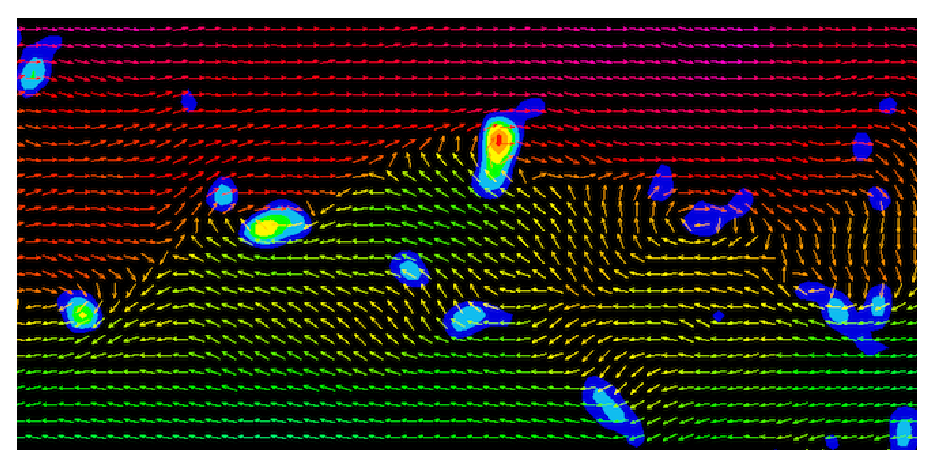
\includegraphics[width=5in]{SampleImage2}
	\caption{Long captions should be fully justified. Figures may appear either at the end of the paper or within the text of the paper.  Color figures are accepted.}
	\label{figure2}
	\end{figure*}


%%%%%%%%%%%%%%%%%%%%%%%%%%%%%%%%%%%%%%%%%%%%%%%%%%%%%%%%%%%%%%%%%%%%%%
\section*{TABLES}

A table should look like Table 1.

\begin{table}[ht]
\centering
\caption{This is an example of a TSFP-10 table.}
\label{Table1}
\begin{tabular}{c c c}
& & \\ % put some space after the caption
\hline
\hline
Re	& $b/a$	& $G$ \\
\hline
450	& 2	& 3.182 \\
475	& 2	& 2.982 \\
500	& 4	& 1.768 \\
\hline
\hline
\end{tabular}
\end{table}

All tables should be numbered consecutively and captioned; the caption should be 9 pt, and upper and lower case letters. It should be placed above the table and centered, if less than one line long, or fully justified if longer. The body of the table should be no smaller than 7 pt. The use of boldface and italics is encouraged to make necessary distinctions within the table. Nine point (9 pt.) leading is recommended.

Tables should be preferably placed at the top of the page in which they are first cross-referenced. Follow the guidelines for figures outlined above for special handling (tables not generated with text, but created separately) and sizes (with specific regard to placement). As with all figures, all tables should be in place on the page when the final paper is submitted. There should be a minimum of two line spaces between tables and text.

%%%%%%%%%%%%%%%%%%%%%%%%%%%%%%%%%%%%%%%%%%%%%%%%%%%%%%%%%%%%%%%%%%%%%%
\section*{REFERENCES}

Within the text, references should be cited by giving the last name of the author(s) and the year of publication of the reference. The year should always be enclosed in parentheses; whether or not the name of the author(s) should be enclosed within the parentheses depends on the context. The two possibilities are illustrated below.

It was shown by Tung (1982) and Lee et al. (1982) that the width of the plume decreases under these conditions.

or

It has been shown that the width of the plume decreases under these conditions (Tung, 1982; Lee et al., 1982).

In the case of two authors, the last names of both authors should be included in the citation, with the word "and" separating the two authors (Kwon and Pletcher, 1981). In the case of three or more authors, only the last name of the first author of the reference should be included, as shown in the above examples, with the other authors being denoted by "et al." In the case of two or more references with the same author(s) and with the same year of publication, the references should be distinguished in the text by appending a lowercase letter "a" to the year of publication of the first cited (Sparrow, 1980a), a letter "b" to the second cited (Sparrow, 1980b), etc.

References to original sources for cited material should be listed together at the end of the paper; footnotes should not be used for this purpose. References should be arranged in alphabetical order according to the last name of the author, or the last name of the first-named author for papers with more than one author. Each reference should include the last name of each author followed by his/her initials. In all cases, titles of books, periodicals, and conference proceedings should be underlined or in italics. A sample list of references in which these forms are illustrated follows.

If you are using BibTeX to manage your bibliography, you can cite an article by typing $\backslash$cite\{citekey\} which will show as \cite{Lee}. \nocite{Kwon} \nocite{Sparrow2} \nocite{Sparrow} \nocite{Tung}

\bibliographystyle{tsfp}
\bibliography{tsfp}
% In this example, BibTeX is used
% For users not familiar with LaTeX, the bibliography can be typed in directly. In this case, comment the two lines above.
%%%%%%%%%%%%%%%%%%%%%%%%%%%%%%%%%%%%%%%%%%%%%%%%%%%%%%%%%%%%%%%%%%%%%%%
%\section*{SAMPLE REFERENCES}
%
%Kwon, O. K., and Pletcher, R. H., 1981, "Prediction of the Incompressible Flow Over a Rearward-Facing Step", Technical Report HTL-26, CFD-4, Iowa State Univ., Ames, IA.
%
%Lee, Y., Korpela, S. A., and Horne, R. N., 1982, "Structure of Multi-Cellular Natural Convection in a Tall Vertical Annulus," Proceedings, 7th International Heat Transfer Conference, U. Grigul et al., ed., Hemisphere Publishing Corp., Washington, D.C., Vol. 2, pp. 221-226.
%
%Sparrow, E. M., 1980a, "Fluid-to-Fluid Conjugate Heat Transfer for a Vertical Pipe - Internal Forced Convection and External Natural Convection", ASME Journal of Heat Transfer, Vol. 102, pp. 402-407.
%
%Sparrow, E. M., 1980b, "Forced-Convection Heat Transfer in a Duct Having Spanwise-Periodic Rectangular Protuberances", Numerical Heat Transfer, Vol. 3, pp. 149- 167.
%
%Tung, C. Y., 1982, Evaporative Heat Transfer in the Contact Line of a Mixture, Ph.D. Thesis, Rensselaer Polytechnic Institute, Troy, NY.

%%%%%%%%%%%%%%%%%%%%%%%%%%%%%%%%%%%%%%%%%%%%%%%%%%%%%%%%%%%%%%%%%%%%%%


\end{document}
